\section{RQ4: What Should Clients Do?}\label{sec:rq4}

A client could respond to drift by asking the user to approve a server again. The question is when. Asking too often produces the warning fatigue documented for browser warnings and mobile permissions~\cite{akhawe2013alice,felt2012android}; asking too rarely leaves approvals that no longer describe the code. We replay the real version histories under six re-approval rules and measure, for each, how often it would prompt and which changes it would surface.

\paragraph{Setup}
We use the 1,667 servers whose observed history spans at least three months, so that per-year rates are meaningful. For each rule we count the version pairs in which it fires and divide by the length of the server's history. Because we sample releases, these rates are lower bounds. As the target, a rule should surface the changes our human annotation judged security-relevant (Section~\ref{sec:rq3}). \todo{Replace proxy target (silent high-risk gains, 420 version pairs) with human-labelled security-relevant changes; update Fig. 6 and the coverage numbers below.}

\paragraph{Results}
Figure~\ref{fig:policies} shows the trade-off. Re-approving on every update surfaces everything but prompts a median of 15.7 times per server per year, and a user typically runs several servers. Re-approving a tool when its own description changes is the rule that matches how clients present tools today, and it prompts 2.4 times per server per year; by construction it surfaces none of the silent gains, which are precisely the changes whose descriptions did not change. Re-approving the whole server whenever any description changes catches about half of them (\todo{update}\%), but only by coincidence: another tool happened to be edited in the same release. Rules keyed to capabilities prompt least, 1.2 times per server per year for any capability and 0.6 for high-risk ones, and target the right changes, but they are only as good as the capability detection behind them, which Section~\ref{sec:rq3} shows is imperfect.

\begin{figure}[t]
\centering
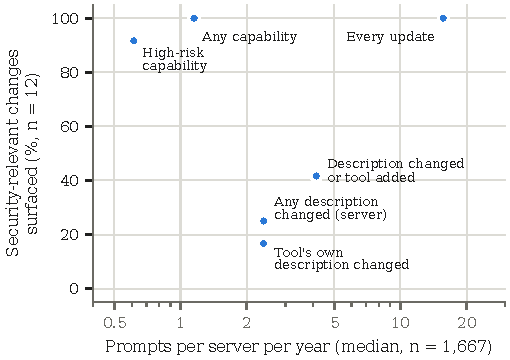
\includegraphics[width=\columnwidth]{figures/fig_policies.pdf}
\caption{Re-approval rules replayed on real histories: median prompts per server per year ($n=1{,}667$ servers with $\geq$3 months of history) against the share of security-relevant changes each rule surfaces. \todo{coverage axis from human labels}}
\label{fig:policies}
\end{figure}

\begin{finding}{4}
Description-based re-approval is cheap but blind to silent capability gains; re-approving on every update is complete but prompts users many times a year. Approval tied to code-derived capabilities prompts least while targeting the changes that matter.
\end{finding}
